\documentclass[../main.tex]{subfiles}
\graphicspath{{\subfix{../images/}}}
\usepackage{subfiles}
\usepackage{subfig}

\begin{document}
    \subsection{Problem Outline}
        Anomaly detection consists on the task of identifying patterns in data that are not consistent with its expected behaviour \cite{chandola2009anomaly}. As such, it is applied in many different areas, from fraud detection in bank transactions all the way to health monitoring systems, as will be shown later in more details. It might be important first to distinguish between anomalies and novelties in the data, with the difference being that the later has patterns that are incorporated into the data after their first appearance. Although anomalies can intuitively be fairly easy to understand (such as the example shown in Figure \ref{fig:anomaly}) there are many challenges related to their actual detection, with some of the most relevant ones being:

        \begin{itemize}
            \item Defining a normal region that actually encompasses every possible normal behaviour;
            \item Anomalous patterns can change with time;
            \item Small quantities of labeled data for training;
            \item Noise in the samples may have similar properties to anomalies;
            \item The actual description of the anomaly is strictly related to the application at hand.          
        \end{itemize}

        \begin{figure}[h]
          \begin{center}
            \centering
            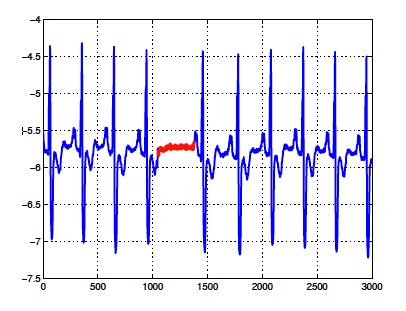
\includegraphics[width={0.6\columnwidth}]{images/ecg_anomaly.png}
            \caption{ECG signal showing the data deemed normal in blue and the anomaly marked in red. In this case, the anomaly correspond to an Atrial Premature Contraction(Image adapted from \cite{chandola2009anomaly})}
          \label{fig:anomaly}
          \end{center}
        \end{figure}

        Anomalies can come in a few different forms. When there is a single instance of the data that has an anomalous behaviour when compared to the rest, it is called a \textbf{point anomaly}. When the anomalous behaviour is only classified as so in a specific context, being considered normal in others, it is called \textbf{contextual} or \textbf{conditional anomaly}. When a collection of related instances is anomalous with respect to the rest of the data (even if those individual instances are not anomalies by themselves) is called a \textbf{collective anomaly}. \par

        Another important distinction to make is in the nature of the available data, that can be either labeled or unlabeled, depending on whether the dataset contains the information on the anomalies locations or not. When choosing an anomaly detection algorithm, this characteristic of the data determines whether a supervised, semi-supervised or unsupervised approach will be used. In supervised learning techniques, we have the data labeled between the normal and anomalous classes and usually train predictive models that classify the new data between the labels. One problem with this approach is that, by the nature of anomalies, datasets are highly biased with normal instances, which might affect the final predictions if not taken into account. In semi-supervised techniques, the dataset contains only one of the classes (usually the normal one), and then a model for this classes behaviour and apply it to see whether the instance follows it or not. The last type possible is unsupervised learning, in which the data available has no labels indicating what samples are normal and what are anomalous, and the model itself has to learn that in its training. The unsupervised models are the most widely applicable precisely because of this property of not requiring training data.

\end{document}